\chapter{Refrigerantes}
\minitoc
\section{Refrigerantes y salmueras}
Un \textbf{refrigerante} es un medio (fluido) para la transferencia de calor que se utiliza en un sistema de refrigeración para absorber calor al evaporarse a temperatura y presión bajas, y ceder el calor al condensarse a temperatura y presión mayores.

La \textbf{salmuera} es un fluido utilizado como refrigerante secundario, transfiriendo el efecto frigorífico desde un circuito primario al espacio requerido.

\section{Nomenclatura}

Cada refrigerante se indica con un color.

El nombre de un refrigerante se representa mediante la letra R seguida de cuatro cifras que indican su composición química. 
\[\text{R}-\text{XXXX}\]
Cada una de estas cifras tiene un significado determinado (de izquierda a derecha):

\begin{enumerate}[label=$X_{\arabic*}$:]
	\item N° de enlaces de carbono no saturados —dobles o triples enlaces—.
	\item N° de átomos de carbono - 1.
	\item N° de átomos de hidrógeno + 1.
	\item N° de átomos de flúor.
\end{enumerate}

Además, en algunos casos, al nombre del refrigerante se le agrega una letra al final (por ejemplo, R-134a). Esta letra indica la \textbf{isomería} del compuesto. La \emph{isomería} es un fenómeno químico por el cual dos compuestos tienen la misma fórmula molecular, es decir, los mismos tipos y cantidades de átomos, pero diferente estructura o disposición espacial.

\section{Clasificación de los refrigerantes}

Los refrigerantes se pueden clasificar de distintas formas, según el criterio:

\begin{itemize}
	\item Según su \textbf{composición química}: orgánicos e inorgánicos, y dentro de estos se tienen los hidrocarburos y los halogenados.
	\item Según su \textbf{comportamiento}: puros, mezclas zeotrópicas o azeotrópicas.
\end{itemize}

\subsection{Clasificación por composición química}

\begin{itemize}
	\item \textbf{Inorgánicos}: no contienen átomos de carbono en su estructura química. Pertenecen a la familia de los refrigerantes R-700. Ejemplos: amoníaco (R-717), agua (R-718), dióxido de carbono (R-744). Su nomenclatura se escribe como \[\text{R-}700 + \text{peso molecular}\]
	\item \textbf{Hidrocarburos}: compuestos únicamente por carbono e hidrógeno. Son naturales y altamente inflamables. Ejemplos: R-290 (propano), R-600 (butano), R-600a (isobutano).
	\item \textbf{Halogenados}: derivados orgánicos que contienen flúor, cloro y/o bromo. Se subdividen en:
	\begin{itemize}
		\item \textbf{CFC (Cloro-Flúor-Carbono)}
		\item \textbf{HCFC (Hidrógeno-Cloro-Flúor-Carbono)}
		\item \textbf{HFC (Hidrógeno-Flúor-Carbono)}
	\end{itemize}
\end{itemize}

\subsection{Clasificación por comportamiento termodinámico}

\begin{itemize}
	\item \textbf{Refrigerantes puros}: formados por un solo compuesto. Cambian de fase a temperatura y presión constantes. Ejemplos: R-134a, R-290, R-744.
	\item \textbf{Mezclas zeotrópicas}: compuestas por dos o más refrigerantes que tienen diferentes puntos de ebullición, por lo tanto, cambian de fase con deslizamiento (\emph{glide}) de temperatura. Pertenecen a la familia R-400. Ejemplo: R-407C.
	\item \textbf{Mezclas azeotrópicas}: se comportan como un refrigerante puro en un punto específico de presión y temperatura. Cambian de fase sin deslizamiento. Pertenecen a la familia R-500. Ejemplo: R-507.
\end{itemize}

\subsection{Clasificación por peligrosidad}

Los refrigerantes se clasifican según su peligrosidad:
\begin{itemize}
	\item \textbf{Inflamabilidad}: números 1, 2, 3.
	\item \textbf{Toxicidad}: letras A y B.
\end{itemize}
\begin{figure}[h]
	\centering
	\caption{Clasificación de los refrigerantes según su peligrosidad, por ASHRAE Standard 34.}
	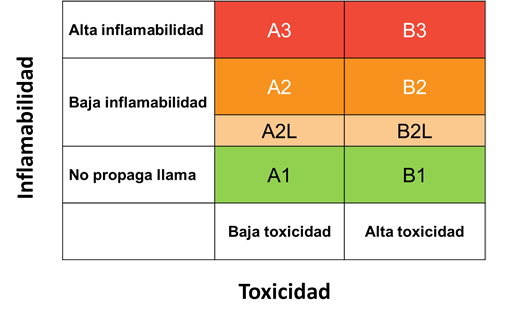
\includegraphics[width=0.5\linewidth]{refrigerantes/peligrosidad-refrigerantes}
\end{figure}

El triángulo Hidrógeno (H), Flúor (F), Cloro (Cl) es una herramienta visual para entender los compromisos y riesgos en la elección de refrigerantes.

\begin{itemize}
	\item Vértice superior: Hidrógeno (H). Aumenta la inflamabilidad de los refrigerantes.
	\item Vértice izquierdo: Cloro (Cl). Aumenta el ODP (Potencial de Destrucción del Ozono) y la toxicidad.
	\item Vértice derecho: Flúor (F). Disminuye la toxicidad, pero aumenta el GWP (Potencial de Calentamiento Global). Contribuye a la larga duración en la atmósfera.
\end{itemize}

\begin{figure}[H]
	\centering
	\caption{Triángulo H-F-Cl.}
	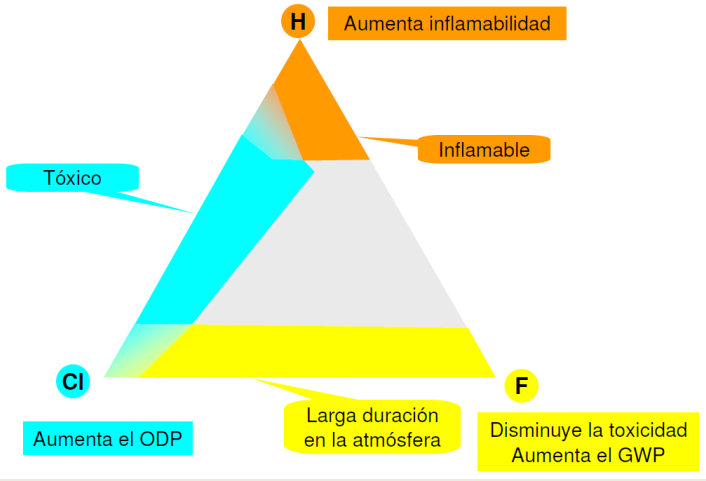
\includegraphics[width=0.6\linewidth]{refrigerantes/triangulo}
\end{figure}
\section{Código de colores}
Aunque fue muy usado durante años, AHRI (Air-Conditioning, Heating, and Refrigeration Institute) dejó de recomendar el uso del código de colores para cilindros a partir del 1 de enero de 2020 debido a las confusiones que ocasionaba, a las complejas mezclas que existen y a los errores que se podían cometer en el pintado.
\begin{figure}[H]
	\centering
	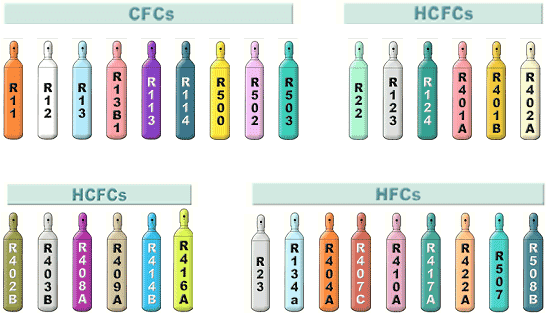
\includegraphics[width=\linewidth]{refrigerantes/codigo-colores}
	\caption{Código de colores para los cilindros de refrigerantes.}
\end{figure}
\section{Requisitos de los refrigerantes}

\begin{itemize}
	\item \textbf{Presiones}: la presión de condensación debe estar muy por debajo de la crítica, debido a bajos calores latentes, además, no tiene una distinción clara entre fase líquida y gaseosa. La presión de evaporación debe estar por encima de la atmosférica, para que no haya filtraciones e ingrese aire exterior.
	\item \textbf{Calor latente de vaporización}: es el calor que absorberá. Representado por una horizontal en el diagrama de Mollier.
	\item \textbf{Calor latente de condensación}: es el calor que cederá al exterior. Representado por una horizontal en el diagrama de Mollier, por encima del de vaporización.
	\item \textbf{Temperatura}: no debe ser excesivamente alta para evitar la descomposición del lubricante —y daños en el compresor—.
	\item \textbf{Punto de congelación}: debe ser bajo, por obvias razones creo yo. Para que no se congele dentro del circuito y se tranque como la caca en el inodoro.
	\item \textbf{Exponente isoentrópico}: debe ser reducido. A mayor exponente, mayor trabajo de compresión necesario. En el diagrama ph se representa como una recta inclinada en la compresión: más inclinada, más energía requiere para comprimirse.
	\item \textbf{Peligrosidad}: no debe ser tóxico ni dañino para personas, componentes del sistema, ni con el medioambiente.
	\item \textbf{Accesibilidad}: debe estar disponible y ser de bajo costo —aguante el capitalismo—.
\end{itemize}

\subsection{Potencial de Calentamiento Global (GWP)}
El GWP (Global Warming Potential) indica cuánto contribuye un gas al calentamiento global comparado con el dióxido de carbono.

\subsection{Potencial de Destrucción del Ozono (ODP)}
El ODP (Ozone Destruction Potential) mide la capacidad de una sustancia para destruir la capa de ozono.



\section{Resumen}

El cuadro presenta un resumen de los refrigerantes más comunes, clasificados por colores según su nivel de uso actual: en rojo, los que están en desuso; en naranja, los que se encuentran en proceso de ser reemplazados; y en verde, los que se utilizan actualmente y continuarán en uso a largo plazo.
\begin{figure}[h]
	\centering
	\caption{Clasificación de los refrigerantes.}
	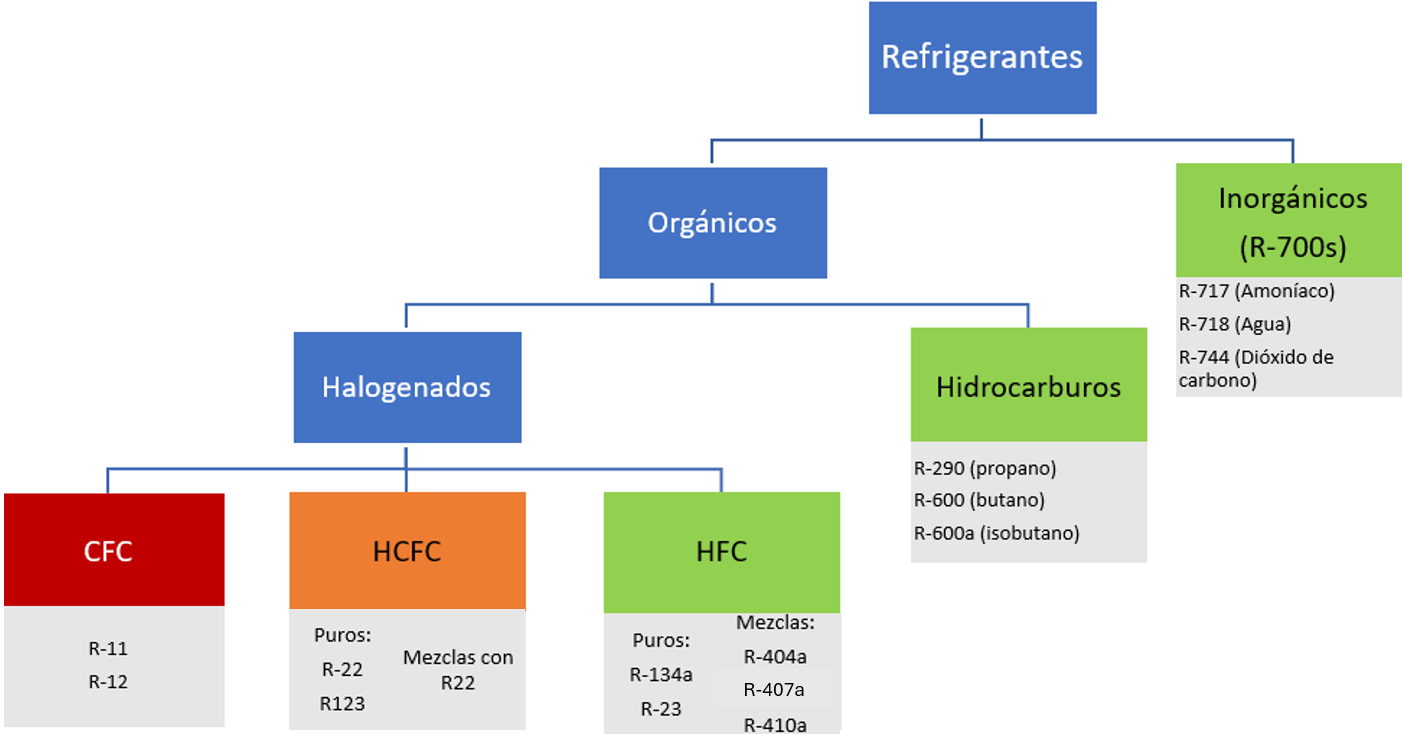
\includegraphics[width=\linewidth]{refrigerantes/resumen}
\end{figure}